\documentclass[a4paper]{article}

\usepackage[utf8]{inputenc}
\usepackage[brazil]{babel}
\usepackage{a4wide}		% correta formatacao da pagina em A4
\usepackage{setspace}		% para a distancia entre linhas
\usepackage{graphicx}
\usepackage{enumerate}

%opening
\title{Lista 2}
\author{Alisson Azzolini \and Anderson Vieira}

\begin{document}

\maketitle

\section{Caixeiro viajante}
Nesta questão, são propostas duas soluções diferentes para o problema clássico do caixeiro viajante, ambas baseadas em algoritmo genético e usando a mesma codificação, mas cada uma utilizando operadores genéticos diferentes. Na primeira implementação, é utilizado o operador de seleção roleta, e na segunda, seleção por torneio binário.

\subsection{Codificação do problema}
Utilizou-se a codificação inteira. Um cromossomo é representado por um vetor de N inteiros não repetidos, cada inteiro de 1 a N representando uma das cidades a percorrer, onde N é o número de cidades. Na solução gerada, as cidades são visitadas na ordem em que aparecem no cromossomo.

\subsection{Instância do problema}

A instância do problema a ser tratada é ilustrada na figura~\ref{fig:otima}. A solução ótima é representada na figura. Esta solução tem comprimento 75.6.

\begin{figure}[h!]
  \centering
%  \input optimal_trip.tex
  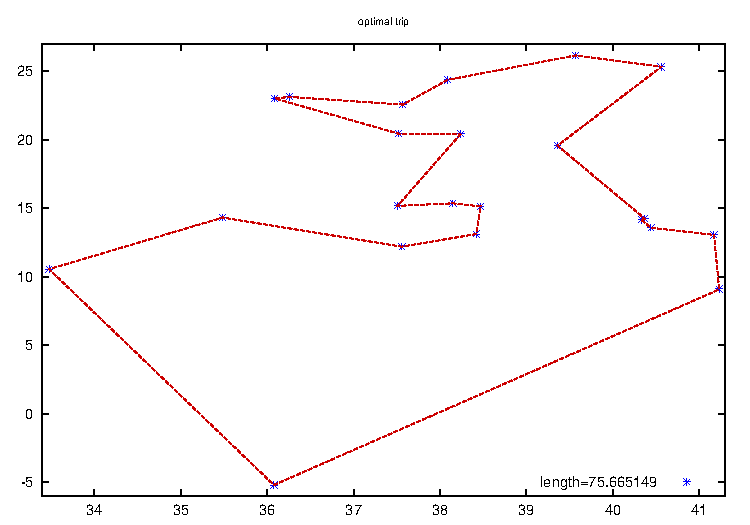
\includegraphics[scale=0.8]{optimal_trip}
  \caption{Instância \textit{Ulysses22}, com a solução ótima fornecida}
  \label{fig:otima}
\end{figure}

\subsection{Solução 1: Roleta}


\subsection{Solução 2: Torneio binário}

Seja $ P_{k} $ o conjunto de indivíduos na geração $ k $. O operador de seleção por torneio seleciona $ m < |P_k| $ indivíduos dessa população, gerando o conjunto $ S_{k} $, da seguinte forma:

\begin{itemize}
 \item faz $ S_{k} = \emptyset $
 \item enquanto $ |S_{k}| < m $
\begin{itemize}
 \item toma indivíduos $ i_1, i_2 \in P_{k} $, aleatoriamente
 \item faz $ S_{k} = S_{k} \cup \arg\max_{\{i_1,i_2\}}\{fitness(i)\} $
\end{itemize}
\end{itemize}

Na implementação realizada, toma-se $ m = {N \over 3} $, $ N = |P_k| $.

De posse dos indivíduos selecionados na k-ésima geração, o algoritmo gera a nova população, $ P_{k+1} $, da seguinte forma:

\begin{itemize}
 \item faz $ P_{k+1} = \emptyset $
 \item enquanto $ |P_{k+1}| < N $
\begin{itemize}
 \item toma $ i_1, i_2 \in S_{k} $, aleatoriamente
 \item com probabilidade $ p_c $, recombina $ i_1 $ e $ i_2 $
 \item com probabilidade $ p_m $, muta $ i_1 $
 \item com probabilidade $ p_m $, muta $ i_2 $
 \item faz $ P_{k+1} = P_{k+1} \cup \{i_1, i_2\} $
\end{itemize}

\end{itemize}



\section{Discussão sobre algoritmos evolutivos}
Nesta questão, discute-se a aplicabilidade e adequabilidade da solução de seis problemas distintos através de algoritmos evolutivos.

\subsection{Problema 1}
Problema com espaço de soluções contínuo e limitado, função de avaliação contínua e derivável e imagem contínua e limitada 


\subsection{Problema 2}
Problema com espaço de soluções contínuo e limitado, função de avaliação contínua mas 
não-derivável e imagem contínua e limitada 

\subsection{Problema 3}
Problema com espaço de soluções contínuo e limitado, função de avaliação descontínua, mas multi-modal com número finito de modos e imagem discreta 

\subsection{Problema 4}
Problema com espaço de soluções discreto, infinito e não-limitado 

\subsection{Problema 5}
Problema com espaço de soluções discreto, infinito mas limitado e função de avaliação multi-modal, com número finito de modos 

\subsection{Problema 6}
Problema com espaço de soluções discreto e finito e função de avaliação multi-modal, com número finito de modos 


\end{document}
 